\documentclass{standalone}
\usepackage{tikz}
\usetikzlibrary{patterns, positioning}


\begin{document}
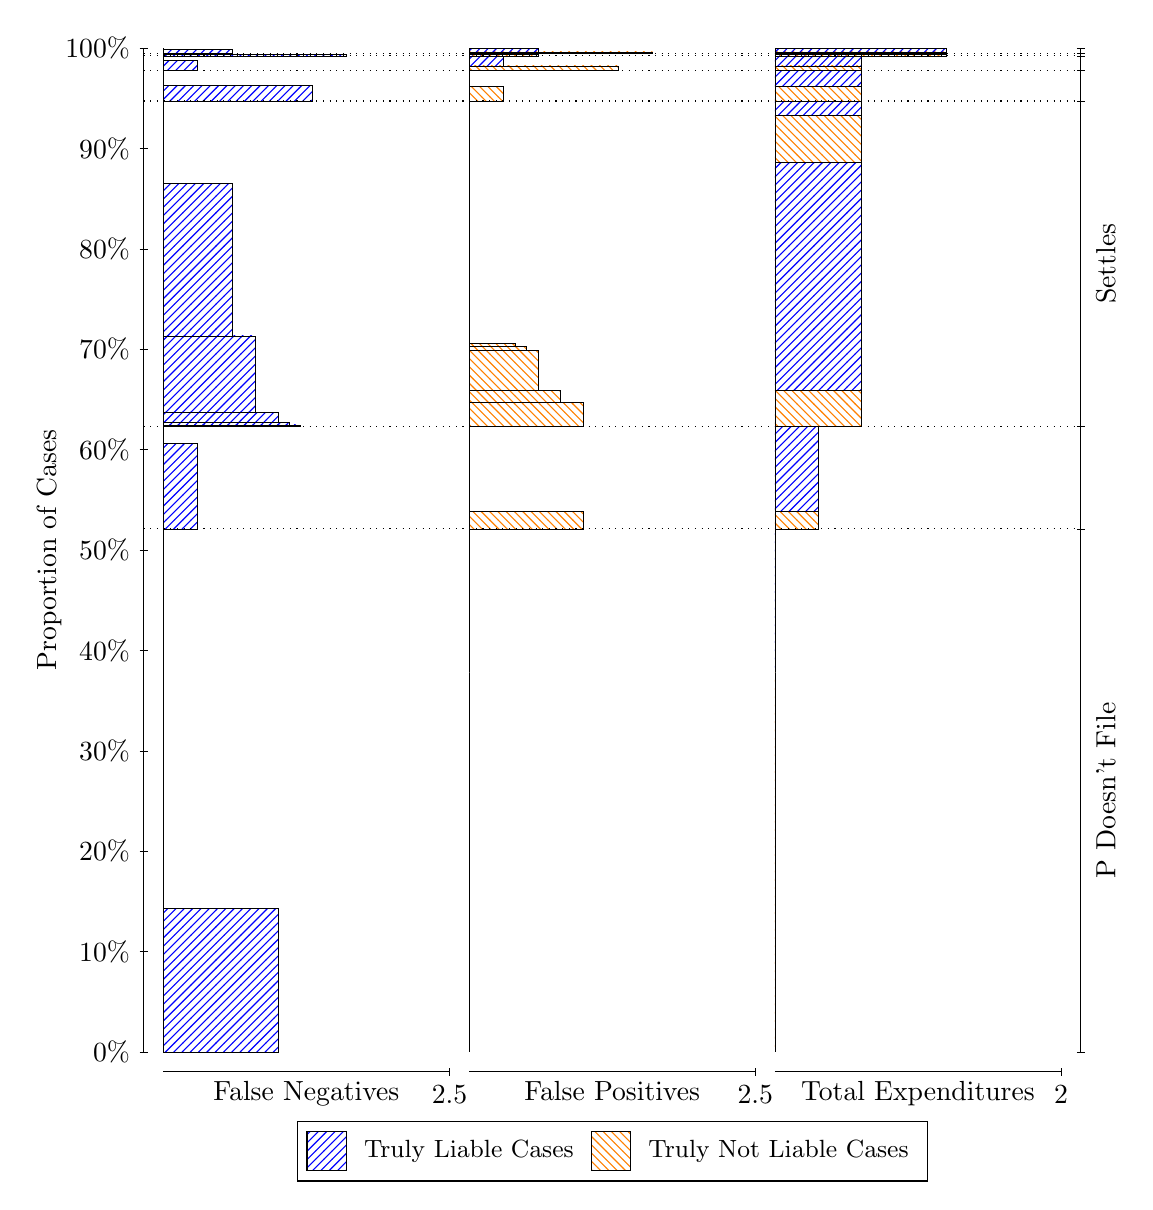
\begin{tikzpicture}
\draw[black, very thin] (1.5,1.75) -- (1.5,14.5);
\node[rotate=90, text=black, anchor=center] at (0.3, 8.125) {Proportion of Cases};
\draw[black, very thin] (1.45,1.75) -- (1.55,1.75);
\node[text=black, anchor=east] at (1.45, 1.75) {0\%};
\draw[black, very thin] (1.45,3.025) -- (1.55,3.025);
\node[text=black, anchor=east] at (1.45, 3.025) {10\%};
\draw[black, very thin] (1.45,4.3) -- (1.55,4.3);
\node[text=black, anchor=east] at (1.45, 4.3) {20\%};
\draw[black, very thin] (1.45,5.575) -- (1.55,5.575);
\node[text=black, anchor=east] at (1.45, 5.575) {30\%};
\draw[black, very thin] (1.45,6.85) -- (1.55,6.85);
\node[text=black, anchor=east] at (1.45, 6.85) {40\%};
\draw[black, very thin] (1.45,8.125) -- (1.55,8.125);
\node[text=black, anchor=east] at (1.45, 8.125) {50\%};
\draw[black, very thin] (1.45,9.4) -- (1.55,9.4);
\node[text=black, anchor=east] at (1.45, 9.4) {60\%};
\draw[black, very thin] (1.45,10.675) -- (1.55,10.675);
\node[text=black, anchor=east] at (1.45, 10.675) {70\%};
\draw[black, very thin] (1.45,11.95) -- (1.55,11.95);
\node[text=black, anchor=east] at (1.45, 11.95) {80\%};
\draw[black, very thin] (1.45,13.225) -- (1.55,13.225);
\node[text=black, anchor=east] at (1.45, 13.225) {90\%};
\draw[black, very thin] (1.45,14.5) -- (1.55,14.5);
\node[text=black, anchor=east] at (1.45, 14.5) {100\%};

\draw[black, very thin] (13.4,1.75) -- (13.4,14.5);
\draw[black, very thin] (13.35,1.75) -- (13.45,1.75);
\node[anchor=west] at (13.35, 1.75) {};
\draw[black, very thin] (13.35,8.3938) -- (13.45,8.3938);
\node[anchor=west] at (13.35, 8.3938) {};
\draw[black, very thin] (13.35,9.6973) -- (13.45,9.6973);
\node[anchor=west] at (13.35, 9.6973) {};
\draw[black, very thin] (13.35,13.827) -- (13.45,13.827);
\node[anchor=west] at (13.35, 13.827) {};
\draw[black, very thin] (13.35,14.213) -- (13.45,14.213);
\node[anchor=west] at (13.35, 14.213) {};
\draw[black, very thin] (13.35,14.4) -- (13.45,14.4);
\node[anchor=west] at (13.35, 14.4) {};
\draw[black, very thin] (13.35,14.436) -- (13.45,14.436);
\node[anchor=west] at (13.35, 14.436) {};
\draw[black, very thin] (13.35,14.5) -- (13.45,14.5);
\node[anchor=west] at (13.35, 14.5) {};

\draw[black, very thin, pattern color=blue, pattern=north east lines] (1.75,1.75) rectangle (3.2033,3.5728);
\draw[black, very thin, pattern color=orange, pattern=north west lines] (1.75,3.5728) rectangle (1.75,8.3938);
\draw[black, very thin, pattern color=blue, pattern=north east lines] (1.75,8.3938) rectangle (2.186,9.4751);
\draw[black, very thin, pattern color=orange, pattern=north west lines] (1.75,9.4751) rectangle (1.75,9.6973);
\draw[black, very thin, pattern color=blue, pattern=north east lines] (1.75,9.6973) rectangle (3.494,9.7144);
\draw[black, very thin, pattern color=blue, pattern=north east lines] (1.75,9.7144) rectangle (3.3487,9.742);
\draw[black, very thin, pattern color=blue, pattern=north east lines] (1.75,9.742) rectangle (3.2033,9.8751);
\draw[black, very thin, pattern color=blue, pattern=north east lines] (1.75,9.8751) rectangle (2.9127,10.843);
\draw[black, very thin, pattern color=blue, pattern=north east lines] (1.75,10.843) rectangle (2.622,12.778);
\draw[black, very thin, pattern color=orange, pattern=north west lines] (1.75,12.778) rectangle (1.75,13.827);
\draw[black, very thin, pattern color=blue, pattern=north east lines] (1.75,13.827) rectangle (3.6393,14.026);
\draw[black, very thin, pattern color=orange, pattern=north west lines] (1.75,14.026) rectangle (1.75,14.213);
\draw[black, very thin, pattern color=blue, pattern=north east lines] (1.75,14.213) rectangle (2.186,14.341);
\draw[black, very thin, pattern color=orange, pattern=north west lines] (1.75,14.341) rectangle (1.75,14.4);
\draw[black, very thin, pattern color=blue, pattern=north east lines] (1.75,14.4) rectangle (4.0753,14.416);
\draw[black, very thin, pattern color=orange, pattern=north west lines] (1.75,14.416) rectangle (1.75,14.436);
\draw[black, very thin, pattern color=blue, pattern=north east lines] (1.75,14.436) rectangle (2.622,14.485);
\draw[black, very thin, pattern color=orange, pattern=north west lines] (1.75,14.485) rectangle (1.75,14.5);
\draw[black, very thin, pattern color=orange, pattern=north west lines] (5.6333,1.75) rectangle (5.6333,6.5711);
\draw[black, very thin, pattern color=blue, pattern=north east lines] (5.6333,6.5711) rectangle (5.6333,8.3938);
\draw[black, very thin, pattern color=orange, pattern=north west lines] (5.6333,8.3938) rectangle (7.0867,8.6161);
\draw[black, very thin, pattern color=blue, pattern=north east lines] (5.6333,8.6161) rectangle (5.6333,9.6973);
\draw[black, very thin, pattern color=orange, pattern=north west lines] (5.6333,9.6973) rectangle (7.0867,9.9981);
\draw[black, very thin, pattern color=orange, pattern=north west lines] (5.6333,9.9981) rectangle (6.796,10.148);
\draw[black, very thin, pattern color=orange, pattern=north west lines] (5.6333,10.148) rectangle (6.5053,10.658);
\draw[black, very thin, pattern color=orange, pattern=north west lines] (5.6333,10.658) rectangle (6.36,10.708);
\draw[black, very thin, pattern color=orange, pattern=north west lines] (5.6333,10.708) rectangle (6.2147,10.747);
\draw[black, very thin, pattern color=blue, pattern=north east lines] (5.6333,10.747) rectangle (5.6333,13.827);
\draw[black, very thin, pattern color=orange, pattern=north west lines] (5.6333,13.827) rectangle (6.0693,14.014);
\draw[black, very thin, pattern color=blue, pattern=north east lines] (5.6333,14.014) rectangle (5.6333,14.213);
\draw[black, very thin, pattern color=orange, pattern=north west lines] (5.6333,14.213) rectangle (7.5227,14.273);
\draw[black, very thin, pattern color=blue, pattern=north east lines] (5.6333,14.273) rectangle (6.0693,14.4);
\draw[black, very thin, pattern color=orange, pattern=north west lines] (5.6333,14.4) rectangle (6.5053,14.421);
\draw[black, very thin, pattern color=blue, pattern=north east lines] (5.6333,14.421) rectangle (5.6333,14.436);
\draw[black, very thin, pattern color=orange, pattern=north west lines] (5.6333,14.436) rectangle (7.9587,14.451);
\draw[black, very thin, pattern color=blue, pattern=north east lines] (5.6333,14.451) rectangle (6.5053,14.5);
\draw[black, very thin, pattern color=orange, pattern=north west lines] (9.5167,1.75) rectangle (9.5167,6.5711);
\draw[black, very thin, pattern color=blue, pattern=north east lines] (9.5167,6.5711) rectangle (9.5167,8.3938);
\draw[black, very thin, pattern color=orange, pattern=north west lines] (9.5167,8.3938) rectangle (10.062,8.6161);
\draw[black, very thin, pattern color=blue, pattern=north east lines] (9.5167,8.6161) rectangle (10.062,9.6973);
\draw[black, very thin, pattern color=orange, pattern=north west lines] (9.5167,9.6973) rectangle (10.607,10.148);
\draw[black, very thin, pattern color=blue, pattern=north east lines] (9.5167,10.148) rectangle (10.607,13.051);
\draw[black, very thin, pattern color=orange, pattern=north west lines] (9.5167,13.051) rectangle (10.607,13.649);
\draw[black, very thin, pattern color=blue, pattern=north east lines] (9.5167,13.649) rectangle (10.607,13.827);
\draw[black, very thin, pattern color=orange, pattern=north west lines] (9.5167,13.827) rectangle (10.607,14.014);
\draw[black, very thin, pattern color=blue, pattern=north east lines] (9.5167,14.014) rectangle (10.607,14.213);
\draw[black, very thin, pattern color=orange, pattern=north west lines] (9.5167,14.213) rectangle (10.607,14.273);
\draw[black, very thin, pattern color=blue, pattern=north east lines] (9.5167,14.273) rectangle (10.607,14.4);
\draw[black, very thin, pattern color=orange, pattern=north west lines] (9.5167,14.4) rectangle (11.697,14.421);
\draw[black, very thin, pattern color=blue, pattern=north east lines] (9.5167,14.421) rectangle (11.697,14.436);
\draw[black, very thin, pattern color=orange, pattern=north west lines] (9.5167,14.436) rectangle (11.697,14.451);
\draw[black, very thin, pattern color=blue, pattern=north east lines] (9.5167,14.451) rectangle (11.697,14.5);
\draw[black, dotted] (1.5,8.3938) -- (13.4,8.3938);
\draw[black, dotted] (1.5,9.6973) -- (13.4,9.6973);
\draw[black, dotted] (1.5,13.827) -- (13.4,13.827);
\draw[black, dotted] (1.5,14.213) -- (13.4,14.213);
\draw[black, dotted] (1.5,14.4) -- (13.4,14.4);
\draw[black, dotted] (1.5,14.436) -- (13.4,14.436);
\draw[black, very thin] (1.75,1.5) -- (5.3833,1.5);
\node[text=black, anchor=north] at (3.5667, 1.5) {False Negatives};
\draw[black, very thin] (5.3833,1.45) -- (5.3833,1.55);
\node[text=black, anchor=north] at (5.3833, 1.45) {2.5};

\draw[black, very thin] (5.6333,1.5) -- (9.2667,1.5);
\node[text=black, anchor=north] at (7.45, 1.5) {False Positives};
\draw[black, very thin] (9.2667,1.45) -- (9.2667,1.55);
\node[text=black, anchor=north] at (9.2667, 1.45) {2.5};

\draw[black, very thin] (9.5167,1.5) -- (13.15,1.5);
\node[text=black, anchor=north] at (11.333, 1.5) {Total Expenditures};
\draw[black, very thin] (13.15,1.45) -- (13.15,1.55);
\node[text=black, anchor=north] at (13.15, 1.45) {2};

\node[text=black, centered, rotate=90] at (13.72, 5.0719) {P Doesn't File};

\node[text=black, centered, rotate=90] at (13.72, 11.762) {Settles};





\draw (7.449999999999999,1.5) node[draw=none] (baseCoordinate) {};
\begin{scope}[align=center]
        \matrix[scale=0.5, draw=black, below=0.5cm of baseCoordinate, nodes={draw}, column sep=0.1cm]{
            \node[rectangle, draw, minimum width=0.5cm, minimum height=0.5cm, pattern color=blue, pattern=north east lines] {}; &
            \node[draw=none, font=\small, text=black] (B) {Truly Liable Cases}; &
            \node[rectangle, draw, minimum width=0.5cm, minimum height=0.5cm, pattern color=orange, pattern=north west lines] {}; &
            \node[draw=none, font=\small, text=black] (B) {Truly Not Liable Cases}; \\
            };
\end{scope}

\end{tikzpicture}
\end{document}